\chapter{Algorytmy i struktury danych}

Materiały teoretyczne zostały opracowane na podstawie slajdów Krzysztofa Diksa. \; \textbf{\red{(przyp. red.: potrzebny link do źródła)}}

\section*{Podstawa programowa}
\begin{enumerate}
    \item Kryteria oceny \textbf{efektywności algorytmów}.
    \item \textbf{Koszt zamortyzowany}.
    \item Podstawowe \textbf{algorytmy sortowania}.
    \item \textbf{Słowniki} i metody ich realizacji.
    \item \textbf{Kolejki priorytetowe} i metody ich realizacji.
\end{enumerate}

\section{Poprawność i efektywność algorytmów}
Powiemy, że algorytm $A$ jest (całkowicie) \textbf{poprawny} względem specyfikacji $\langle \alpha, \beta \rangle$, jeśli spełnia następujące warunki:
\begin{itemize}
    \item \textbf{częściowa poprawność}
    
    Dla każdych danych wejściowych spełniających warunek początkowy $\alpha$, jeśli obliczenie algorytmu $A$ kończy się prawidłowo, wyniki spełniają warunek $\beta$.
    
    \item \textbf{określoność obliczeń}
    
    Dla każdych danych wejściowych spełniających warunek początkowy $\alpha$ obliczenie algorytmu $A$ nie jest przerwane.
    
    \item \textbf{własność stopu}
    
    Dla każdych danych wejściowych spełniających warunek początkowy $\alpha$ obliczenie algorytmu $A$ nie jest nieskończone.
\end{itemize}

\subsection{Złożoność obliczeniowa algorytmu}
Interesują nas dwa typy złożoności:
\begin{itemize}
    \item \textbf{pamięciowa}
    \begin{enumerate}
        \item[a.] ilość pamięci niezbędna do wykonania algorytmu;
        \item[b.] jednostka miary: słowo pamięci maszyny.
    \end{enumerate}
    \item \textbf{czasowa}
    \begin{enumerate}
        \item[a.] czas pracy niezbędny do zrealizowania algorytmu;
        \item[b.] jednostka miary: \textbf{operacja dominująca}, czyli liczba wszystkich operacji jednostkowych wykonywanych przez algorytm powinna być ,,proporcjonalna'' do liczby wszystkich operacji dominujących. Intuicyjnie myślimy o niej jak o operacji, która najbardziej wpływa na czas działania algorytmu. 
    \end{enumerate}
\end{itemize}

Wprowadźmy oznaczenia:
\begin{itemize}
    \item $D_n$ – zbiór możliwych danych wejściowych rozmiaru $n$
    \item $t(d)$ – liczba operacji dominujących dla zestawu danych $d$
    \item $X_n$ – zmienna losowa, której wartością jest $t(d)$ dla $d \in D_n$
    \item $E[X_n]$ - wartość oczekiwana $X_n$
    \item $p_{n,k}$ - prawdopodobieństwo, że dla danych rozmiaru $n$ algorytm wykona $k$ operacji dominujących
\end{itemize}

Przez \textbf{pesymistyczną} złożoność czasową algorytmu rozumie się funkcję
\begin{align*}
    W(n) = \sup \{t(d): d \in D_n\}
\end{align*}

Przez \textbf{oczekiwaną} złożoność czasową algorytmu rozumie się funkcję
\begin{align*}
    A(n) = \sum_{k \geq 0} k \cdot p_{n, k} = E[X_n]
\end{align*}

Intuicyjnie, pesymistyczna złożoność czasowa opisuje zachowanie algorytmu w najgorszym możliwym przypadku, natomiast oczekiwana złożoność czasowa zachowanie w przeciętnym przypadku.
\bigskip

\textbf{Algorytm w miejscu} poza pamięcią na przechowywanie danych, potrzebuje tylko dodatkowej pamięci stałego rozmiaru niezależnie od rozmiaru danych. 

\textbf{Algorytm stabilny} zachowuje względny porządek elementów o tych samych wartościach (np. przy sortowaniu nie zamienia miejscami takich samych elementów).

\begin{example}
    Obliczymy złożoność czasową sortowania przez wstawianie (ang. \textit{insertion sort}). Na wejściu dana jest tablica $a[1...n]$, którą chcemy posortować.
    \begin{cpp}
        a[0] = -INF;              // strażnik, dostatecznie mała wartość
        for (int i = 2; i <= n; i++) {
            v = a[i];
            j = i - 1;
            while (v < a[j]) {    // operacja dominująca
                a[j + 1] = a[j];
                j = j - 1;
            }
            a[j + 1] = v;
        }
    \end{cpp}
    Inwersja w ciągu $a$ to para indeksów $(i, j)$, $1 \leq i < j \leq n$, taka że $a[i] > a[j]$, czyli że element większy znajduje się przed mniejszym. Liczbę inwersji w tablicy $a$ oznaczamy przez $\text{Inv}(a)$. W oczywisty sposób zachodzi $0 \leq \text{Inv}(a) \leq \frac{1}{2}n(n - 1)$.
    
    Złożoność czasowa algorytmu sortowania przez wstawianie mierzona liczbą wykonania operacji dominującej \texttt{v < a[j]}, wynosi $n - 1 + \text{Inv}(a)$, ponieważ dla każdej inwersji $(i, j)$ wykonamy zamianę miejscami elementów $a[i], a[j]$. Dodatkowo, przed wyjściem z pętli \texttt{while} wykonamy jedno porównanie, które nie będzie spełniało warunku pętli.

    Z tego wynika, że pesymistyczna złożoność czasowa algorytmu sortowania przez wstawianie wynosi
    \begin{align*}
        W(n) = n - 1 + \frac{1}{2} \cdot n \cdot (n-1)
    \end{align*}
    Insertion sort jest algorytmem w miejscu oraz stabilnym.
\end{example}

\subsection{Notacja asymptotyczna}
Rozważamy funkcje o argumentach będących nieujemnymi liczbami całkowitymi i o nieujemnych, rzeczywistych wartościach.
\begin{itemize}
    \item Dla danej funkcji $g(n)$ przez $\purple{O(g(n))}$ oznaczamy zbiór funkcji
    \begin{align*}
        O(g(n)) = \{f(n): \text{ istnieją dodatnie stałe } c, n_0 \text{, takie że } \forall_{n \geq n_0} \; 0 \leq f(n) \leq c \cdot g(n) \}
    \end{align*}
    Piszemy $f(n) = O(g(n))$, gdy $f(n) \in O(g(n))$. Możemy o tym myśleć jak o \textbf{ograniczeniu z~góry} tempa wzrostu $f$ przez $g$, podobnie jak to robimy na analizie matematycznej.

    \item Dla danej funkcji $g(n)$ przez $\purple{\Omega(g(n))}$ oznaczamy zbiór funkcji
    \begin{align*}
        \Omega(g(n)) = \{f(n): \text{ istnieją dodatnie stałe } c, n_0 \text{, takie że } \forall_{n \geq n_0} \; 0 \leq c \cdot g(n) \leq f(n) \}
    \end{align*}
    Piszemy $f(n) = \Omega(g(n))$, gdy $f(n) \in \Omega(g(n))$. Możemy o tym myśleć jak o notacji przeciwnej do $O$, a więc jak o \textbf{ograniczeniu z~dołu} tempa wzrostu $f$ przez $g$.

    \item Dla danej funkcji $g(n)$ przez $\purple{\Theta(g(n))}$ oznaczamy zbiór funkcji
    \begin{align*}
        \Theta(g(n)) = \{f(n): \text{ istnieją dodatnie stałe } c_1, c_2, n_0 \text{, takie że } \forall_{n \geq n_0} \; 0 \leq c_1 \cdot g(n) \leq f(n) \leq c_2 \cdot g(n) \}
    \end{align*}
    Piszemy $f(n) = \Theta(g(n))$, gdy $f(n) \in \Theta(g(n))$. Oznacza to, że tempo wzrostu $f$~i~$g$~jest takie samo, a więc zachodzi jednocześnie $f(n) = \Omega(g(n))$ oraz $f(n) = O(g(n))$.
\end{itemize}

\begin{example}
    Kontynuujemy przykład z algorytmem insertion sort. Przypomnijmy obliczoną wcześniej złożoność pesymistyczną:
    \begin{align*}
        W(n) = n - 1 + \frac{1}{2} \cdot n \cdot (n-1) = \frac{n^2}{2} + \frac{n}{2} - 1 
    \end{align*}
    Dzięki notacji asymptotycznej możemy więc powiedzieć, że pesymistyczna złożoność algorytmu insertion sort to $\Theta(n^2)$.

    Obliczmy złożoność oczekiwaną $A(n)$. Dla każdej pary różnych indeksów $i, j$ utworzą one inwersję z prawdopodobieństwem równym $\frac{1}{2}$. Z niezależności wartości oczekiwanej uzyskujemy
    \begin{align*}
        A(n) = n - 1 + \frac{1}{2} \cdot \frac{1}{2} \cdot n \cdot (n-1) = \frac{n^2}{4} + \frac{3n}{4} - 1
    \end{align*}
    Zatem oczekiwana złożoność algorytmu insertion sort to również $\Theta(n^2)$.
\end{example}

% TODO
\begin{editorsnote}
    W części teoretycznej brak informacji o koszcie zamortyzowanym, jednak zawarta tu teoria jest wystarczająca do rozwiązania zadań z przeanalizowanych na potrzeby tego repetytorium archiwalnych egzaminów.
\end{editorsnote}

\begin{problems}
    \prob Agata i Bartek grają w grę polegającą na tym, że Agata wybiera dwie liczby ze zbioru $\{1, 2, ..., n\}$, a Bartek zadaje pytania o wybrany podzbiór i dowiaduje się, czy co najmniej jedna z wybranych liczb znajduje się w nim. Liczba zapytań wystarczających do określenia przez Bartka obu liczb jest
    \answers{$O(n)$}{$O(\sqrt{n})$}{$O(\log{n})$}
\end{problems}

\section{Kolejki priorytetowe}

\textbf{Kopiec} to struktura danych oparta na drzewie. We wszystkich wierzchołkach trzymamy wartości, zwane \textbf{kluczami}.
Wartość w rodzicu wierzchołka jest zawsze mniejsza (lub zawsze większa) od wartości potomka.

% TODO
\begin{editorsnote}
    Brakuje tu opisu kopca binarnego, a pojawia się on w dalszej części teorii.
\end{editorsnote}

\subsection{Kopiec zupełny}

\textbf{Kopiec zupełny} to kopiec binarny, w którym liście występują tylko na ostatnim i przedostatnim poziomie, spójnie ułożone od lewej do prawej. Jego wysokość zatem jest rzędu $O(\log n)$, gdzie $n$ to liczba wierzchołków.

Operacja dodania elementu do takiego kopca polega w uproszczeniu na:
\begin{itemize}
    \item Jeśli dodawany element jest większy (zakładamy typ MAX) od korzenia, to zamieniamy je. W wyniku tej operacji wciąż mamy jeden element do dołożenia do poddrzewa. 
    \item Wyliczamy, czy nadmiarowy element powinien trafić do lewego czy prawego poddrzewa, żeby utrzymać ,,zupełność'' kopca.
    \item Rekurencyjnie dodajemy element do wybranego poddrzewa.
\end{itemize}

Wierzchołki kopca ponumerujemy od $1$ do~$n$, tak że ojcem wierzchołka $i$ jest wierzchołek o numerze $\lfloor \frac{i}{2} \rfloor$, a~$2i$ oraz $2i + 1$ to odpowiednio jego lewy i prawy syn (o ile istnieją). Wartości w wierzchołkach będziemy trzymać w tablicy $a$.

Jeśli wierzchołki o numerach $[l + 1, \dots, r]$ spełniają własność kopca,
to następująca procedura sprawi, że będzie ją spełniać też wierzchołek $l$.
\begin{cpp}
    void DownHeap(l, r) {
        int i = l, j = 2 * i, v = a[i];
        while (j <= r) { // dopóki istnieje syn wierzchołka
            // sprawdzamy, czy prawy syn ma większą wartość
            if (j + 1 <= r && a[j] < a[j + 1])
               j = j + 1; 
    
            // czy nie spełnia wartości kopca?
            if (v < a[j]) {
                // podnosimy wartość z syna 
                a[i] = a[j]; 
                // schodzimy niżej
                i = j;
                j = 2 * i;
            } else {
                // wszystko jest okej
                break;
            }
        }
        a[i] = v;
    }
\end{cpp}

\subsection{Kopiec dwumianowy (kolejka dwumianowa)}

\textbf{Drzewo dwumianowe} $B_k$ jest zdefiniowane rekurencyjnie. Jest to drzewo $B_{k - 1}$ z drugim drzewem $B_{k - 1}$ przyłączonym krawędzią do korzenia.
Drzewo $B_0$ składa się z pojedynczego wierzchołka. Widać zatem, że $|B_k| = 2^k$.

\begin{figure}[H]
    \centering
    \includegraphics[scale=0.5]{rozdziały/images/ASD/drzewa_dwumianowe.png}
    \caption{Drzewa dwumianowe}
\end{figure}

\textbf{Kolejka dwumianowa} składa się z lasu drzew dwumianowych o parami różnych rozmiarach, których rozmiary w sumie dają $n$. W każdym drzewie elementy są rozmieszczone tak, żeby wartości spełniały porządek kopcowy.

Dostęp do najmniejszego elementu obywa się przez wskaźnik na korzeń z najmniejszą wartością.

W takiej kolejce ważne są dwie operacje:
\begin{itemize}
    \item Join($T_1$, $T_2$) łączy dwa drzewa tego samego stopnia w jedno drzewo o stopniu o 1 większym z zachowaniem porządku kopcowego. Złożoność: $O(1)$.
    \item Union($Q_1$, $Q_2$) łączy dwie kolejki dwumianowe $Q_1, Q_2$ w jedną kolejkę $Q_1$, korzystając z operacji Join. Złożoność: $O(\log n)$.
\end{itemize}

Powyższe operacje wykorzystuje się, żeby zaimplementować kolejkę priorytetową. Na przykład, wstawienie elementu do kolejki to Union() z jednoelementową kolejką.

\subsection{Kopiec Fibonacciego}

\textbf{Kopiec Fibonacciego} składa się z listy dwukierunkowej korzeni kolejnych drzew, tym razem już może być wiele drzew o tych samych rozmiarach. Utrzymywany jest wskaźnik na korzeń z najmniejszą wartością.

Operacja znajdowania minimum jest zatem trywialna, i działa w czasie stałym.

Wstawianie elementu polega na stworzeniu nowego jednoelementowego drzewa i dodaniu go do listy.

Operacja usunięcia najmniejszego elementu przebiega w 3 fazach.
\begin{enumerate}
    \item Usuwamy korzeń zawierający minimalny element, a jego dzieci (z poddrzewami) dołączamy do listy drzew kopca.
    \item Musimy uaktualnić wskaźnik na minimalny klucz. Na liście korzeni może być $n$ elementów, zatem najpierw będziemy łączyć drzewa o tym samym stopniu (liczba synów korzenia).
    \item Uaktualniamy wskaźnik na minimum.
\end{enumerate}
Amortyzowany koszt tej operacji to $O(\log n)$. Jeśli wcześniej wykonywaliśmy same operacje dodawania wierzchołków i usuwania minimum, to otrzymamy w wyniku tej operacji kopiec dwumianowy.

Operacja zmniejszenia wartości (używana w opisanym później algorytmie Dijkstry) zaczyna od zmniejszenia wartości zadanego wierzchołka
i w razie, gdy nowa wartość zaburza porządek kopcowy (wierzchołek ma wartość mniejszą niż rodzic), wywołujemy operację odcinania rozważanego wierzchołka.

Operacja odcinania wierzchołka $x$ odcina go od ojca $y$ i dołącza do listy korzeni kopca. Dodatkowo, $y$ zostaje oznaczony jako wierzchołek, który utracił jedno dziecko. 
Przy próbie odcięcia drugiego dziecka, nie odcinamy go, tylko wywołujemy $cut(y)$, przenosząc operację w górę drzewa tak długo, aż dojdziemy do korzenia, lub wierzchołka który nie utracił jeszcze syna.

Dzięki tym operacjom otrzymujemy koszt amortyzowany $O(1)$ operacji zmniejszenia wartości klucza.

Nazwa kopca pochodzi od tego, że minimalny rozmiar drzewa o stopniu $d$ to liczba Fibonacciego o indeksie $(d + 2)$

\begin{figure}[H]
    \centering
    \includegraphics[scale=0.5]{rozdziały/images/ASD/kopiec_fibonacciego.png}
    \caption{Drzewa o najmniejszym możliwym rozmiarze w kopcu Fibonacciego}
\end{figure}

\subsection{Porównanie}

Zestawienie złożoności najważniejszych operacji (złożoności oznaczone gwiazdką są amortyzowane):

\begin{tabular}{ |l|c|c|c| }
    \hline
    operacja & kopiec zupełny & kopiec dwumianowy  & kopiec Fibonacciego \\
    \hline
    inicjalizacja pustego kopca & $O(1)$ & $O(1)$ & $O(1)$ \\
    \hline
    podanie najmniejszego elementu & $O(1)$ & $O(1)$ & $O(1)$ \\
    \hline
    usunięcie najmniejszego elementu & $O(\log n)$ & $O(\log n)$ & $O(\log n)$* \\
    \hline
    wstawienie elementu & $O(\log n)$ & $O(\log n)$ & $O(1)$* \\
    \hline
    zmniejszenie jednej wartości & $O(\log n)$ & $O(\log n)$ & $O(1)$* \\
    \hline
\end{tabular}

\begin{problems}
    \prob Do początkowo pustego kopca Fibonacciego typu min wstawiamy kolejno rekordy o priorytetach odpowiednio $1, 2, ..., 2020$, otrzymując kopiec $T$, a następnie wykonujemy operację \texttt{DeleteMin}, otrzymując kopiec $T'$. Wynika z tego, że
    \answers{kopiec $T$ składa się z co najwyżej 8 drzew}{kopiec $T'$ składa się z co najwyżej 8 drzew}{najwyższe drzewo w kopcu $T'$ ma wysokość (tzn. największą możliwą liczbę krawędzi od korzenia do liścia w drzewie) co najmniej $10$}
\end{problems}


\section{Algorytmy sortowania}
\subsection{Insertion sort}
Inaczej sortowanie przez wstawianie, opisane powyżej. Cechy:
\begin{itemize}
    \item w miejscu
    \item stabilny
    \item złożoność zależna od liczby inwersji
    \item oczekiwana oraz pesymistyczna złożoność kwadratowa
\end{itemize}

\subsection{Bubble sort}
Inaczej sortowanie bąbelkowe.
\begin{cpp}
    for (int i = n; i >= 2; i--) {
        for (int j = 1; j <= i - 1; j++) {
            if (a[j] > a[j + 1])       // #porównania - wszystkie możliwe czyli n * (n - 1) / 2
                swap(a[j], a[j + 1]);  // #zamiany = Inv(a)
        }
    }
\end{cpp}
Cechy:
\begin{itemize}
    \item w miejscu (+);
    \item stabilny (+);
    \item liczba zamian zależna od liczby inwersji (+/-);
    \item kwadratowa liczba porównań, niezależnie do danych (-).
\end{itemize}

\subsection{Selection sort}
Inaczej sortowanie przez wybieranie.
\begin{cpp}
    for (int i = n; i >= 2; i--) {
        i_max = 1;
        for (int j = 2; j <= i; j++) {
            if (a[j] > a[i_max])   // #porównania = n * (n - 1) / 2
                i_max := j;
        }
        swap(a[i], a[i_max]);  // #zamiany = n - 1
    }
\end{cpp}
Cechy:
\begin{itemize}
    \item w miejscu (+);
    \item nie jest stabilny (-);
    \item mała liczba zamian (+);
    \item kwadratowa liczba porównań, niezależnie do danych (-).
\end{itemize}

\subsection{Heap sort}
Inaczej sortowanie przez kopcowanie. Dzięki użyciu kopca otrzymujemy szybszy selection sort, ponieważ umiemy znajdować maksimum w logarytmicznym czasie.
\begin{cpp}
    // Budowa kopca.
    // Zauważmy, że n / 2 wartości w liściach może zostać przepisanych z tablicy a.
    for (int i = n / 2; i >= 1; i--)
        DownHeap(i, n);

    // Niezmiennik: a[1..i] <= a[i+1] <= ... <= a[n] oraz heap(1,i).
    for (int i = n; i >= 2; i--) {
        swap(a[1], a[i]);
        DownHeap(1, i - 1);
    }
\end{cpp}
Cechy:
\begin{itemize}
    \item w miejscu (+);
    \item nie jest stabilny (-);
    \item pesymistyczny czas działania $\Theta(n \log n)$ (+).
\end{itemize}

\subsection{Merge sort}
Inaczej sortowanie przez scalanie.
\begin{cpp}
    // b[1..n] – globalna tablica pomocnicza
    // Niezmiennik: przy wywołaniu funkcji posortowane jest a[l...s] oraz a[s+1...r].
    // Po wywołaniu posortowane będzie a[l...r].
    void merge(int l, int r, int s) {
        i = l;
        j = s + 1;
        k = l - 1;
        while (i <= s && j <= r) {
            k = k + 1;
            if (a[i] <= a[j]) {     // #porównania <= r - l
                b[k] = a[i];
                i = i + 1;
            }
            else {
                b[k] = a[j];
                j = j + 1;
            }
        }
        if (i > s)
            b[k+1...r] = a[j...r]
        else
            b[k+1...r] = a[i...s]
        a[l...r] = b[l...r]
    }

    void merge_sort(int l, int r) {
        if (l < r) {
            s = (l + r) / 2;
            merge_sort(l, s);
            merge_sort(s + 1, r);
            merge(l, r, s);
        }
    }

    merge_sort(1, n);
\end{cpp}

Cechy:
\begin{itemize}
    \item nie jest w miejscu (-) aczkolwiek istnieje trudniejsza wersja w miejscu;
    \item stabilny (+);
    \item pesymistyczny czas działania $\Theta(n \log n)$ (+);
    \item bardzo mało porównań (+);
    \item sporo przypisań, możliwa redukcja (-/+).
\end{itemize}

\subsection{Quick sort}
Intuicyjnie jest to algorytm, które po prostu buduje drzewo BST.
\begin{cpp}
    // Niech S będzie zbiorem, który chcemy posortować.
    // elem S zwraca wszystkie elementy zbioru S.
    void quick_sort(S) {
        if (|S| <= 1) {
            print(elem S);                       // jedyny element zbioru S
        }
        else {
            x = pivot(S);                        // element dzielący
            S_less = {y: elem S && y < x};       // zbiór elementów mniejszych niż x
            S_greater = {y: elem S && y > x};    // zbiór elementów większych niż x
            quick_sort(S_less);
            print(x);
            quick_sort(S_greater);
        }
    }
\end{cpp}

\begin{figure}[H]
    \centering
    \includegraphics[scale=0.3]{rozdziały/images/ASD/quick_sort.png}
    \caption{Ilustracja działania algorytmu quick sort.}
\end{figure}

W powyższym przykładzie jako pivot wybieramy zawsze pierwszy element sortowanego zbioru. Takie drzewo obliczeń może być niskie (wysokości $O(\log n)$) lub wysokie (np. dla $S = \{1, 2, ..., n\})$. Przy losowym wyborze pivota algorytm ten działa jednak w oczekiwanej złożoności $\Theta(n \log n)$.

Cechy:
\begin{itemize}
    \item prawie w miejscu (-/+);
    \item nie jest stabilny (-);
    \item pesymistyczna złożoność $\Theta(n^2)$ (-);
    \item oczekiwana złożoność $\Theta(n \log n)$ (+);
    \item bardzo dobrze sprawdza się w praktyce.
\end{itemize}

\subsection{Count sort}
Inaczej sortowanie przez zliczanie. Działa dobrze przy założeniu, że elementy tablicy $a$ nie są zbyt duże.
\begin{cpp}
    // b - tablica zliczająca liczbę wystąpień elementów a
    m = max(a) + 1;
    b = [0] * m;
    for (int i = 1; i <= n; i++)
        b[a[i]]++;

    // Dla każdej wartości tablicy a wyznaczamy ostatnią pozycję,
    // na której wystąpi ona w posortowanej tablicy.
    for (int i = 1; i <= m - 1; i++)
        b[i] += b[i - 1];

    // t - tablica pomocnicza
    for (int i = n; i >= 1; i--) {
        t[b[a[i]]] = a[i];
        b[a[i]]--;
    }

    a = t;
\end{cpp}
Cechy:
\begin{itemize}
    \item nie jest w miejscu (-);
    \item stabilny (+);
    \item złożoność $\Theta(n + m)$ (-/+);
    \item dla $m = O(n)$ algorytm liniowy (+).
\end{itemize}

\subsection{Bucket sort}
Inaczej sortowanie kubełkowe. Idea taka sama jak w count sorcie, ale utrzymujemy tablicę list zamiast zwykłego countera.
\begin{cpp}
    // Inicjacja pustych kubełków.
    m = max(a) + 1;
    b = {} * m;
    
    // Wypełnienie kubełków.
    for (int i = 1; i <= n; i++)
        b[a[i]].push_back(a[i]);

    // Końcowe scalenie
    wynik = {};
    for (int i = 0; i <= m - 1; i++)
        wynik.append(b[i]);
\end{cpp}
Cechy:
\begin{itemize}
    \item nie jest w miejscu (-);
    \item stabilny (+);
    \item złożoność $\Theta(n + m)$ (-/+);
    \item dla $m = O(n)$ algorytm liniowy (+).
\end{itemize}

\subsection{Sortowanie leksykograficzne słów tej samej długości}
Dane:
\begin{itemize}
    \item dodatnie liczby całkowite $n, k, m$;
    \item $s[1..n]$ - tablica słów o długości $k$ nad alfabetem $\{0, 1, ..., m - 1\}$;
    \item oznaczenie: $s[i][j]$ – $j$-ta litera w słowie $s[i]$. 
\end{itemize}
Wynik:
\begin{itemize}
    \item $w[1...n]$ – permutacja indeksów $1, ..., n$ wyznaczająca porządek leksykograficzny słów $s$.
\end{itemize}
\begin{cpp}
    w[1...n] = [1, 2, ..., n];
    for (int j = k; j >= 1; j--) {
        posortuj w stabilnie w względem znaków z pozycji j w słowach;
    }
\end{cpp}
Do posortowania stabilnie możemy wykorzystać bucket sort.

Cechy:
\begin{itemize}
    \item stabilny (+);
    \item złożoność $\Theta(k \cdot (n + m))$ (-/+).
\end{itemize}

\subsection{Sortowanie leksykograficzne}
Poprzedni algorytm da się uogólnić na sortowanie leksykograficzne słów różnej długości.

Cechy:
\begin{itemize}
    \item złożoność $\Theta(k \cdot n + m)$ (-/+).
\end{itemize}

\subsection{Inne algorytmy sortowania}
\begin{itemize}
    \item Metoda Shella, usprawnienie insertion sorta, $h$-sortowania.
    \item Sortowanie introspektywne - quick sort z pesymistyczną złożonością $O(n \log n)$.
\end{itemize}

\subsection{Ważny fakt}
Każdy algorytm sortujący \textbf{przez porównania} wykonuje w pesymistycznym przypadku $\Theta(n \log n)$ porównań.


\begin{problems}
    \prob W modelu losowej permutacji, złożoność $\Omega(n^2)$ ma algorytm
    \answers
    {quick sort}
    {insertion sort}
    {heap sort}

    \prob Pesymistyczna złożoność algorytmów sortowania w zależności od liczby inwersji $inv$ to
    \answers{dla insertion sort: $O(\max(n, inv))$}{dla quick sort: $O(n \cdot \log(\max(n, inv)))$}{dla heap sort: $O(n \cdot \log(\max(n, inv)))$}
    
    \prob Ciąg $\delta=\langle\delta_1,\delta_2,\ldots,\delta_n\rangle$ nazywamy $k$-uporządkowanym rosnąco, gdy każdy jego podciąg złożony z~elementów odległych o $k$ jest uporządkowany rosnąco, tzn. $\delta_i<\delta_{i+k}$ dla $i=1,2,\ldots n-k$. Ciąg $\delta$ można uporządkować za pomocą $O(n)$ porównań, gdy jest on
    \answers{jednocześnie 2- i 3-uporządkowany}{2012-uporządkowany}{$\lfloor\log{n}\rfloor$-uporządkowany}
    
    \prob Rozważmy równanie rekurencyjne $$ T(n) = \begin{cases} n & \text{dla }  \; n \leq 1 ,\\ T(\lfloor n/2 \rfloor) + T(\lceil n/2 \rceil ) + n + 1 & \text{dla } \; n > 1 \end{cases} $$
    Wartość $T(n) $
    \answers
    {jest ograniczeniem górnym na liczbę porównań wykonywanych w algorytmie sortowania $n$ różnych elementów przez scalanie}
    {jest ograniczeniem górnym na średnią liczbę porównań w algorytmie sortowania szybkiego dla $n$ różnych elementów, gdy element dzielący jest wybierany losowo z rozkładem jednostajnym}
    {jest rzędu $\Theta (n \log n)$}
\end{problems}

\section{Algorytmy grafowe}

\textbf{Algorytm Dijkstry} w spójnym grafie z krawędziami o nieujemnych wagach szuka najkrótszych ścieżek od wyróżnionego wierzchołka do wszystkich pozostałych.

Pseudokod:
\begin{cpp}
/* s - wierzchołek startowy
 * L - zbiór wierzchołków, dla których znamy już najkrótsze ścieżki
 * R - dopełnienie L
 * w(u, v) - waga krawędzi u -> v
 * N(v) - sąsiedzi wierzchołka v */
begin
    /* inicjacja */
    d(s) := 0, L := {s}, R := V - {s};
    for v in R do d(v) := +inf;
    for v in N(s) do d(v) := w(s, v);

    /* pętla główna */
    while |R| > 0 do
    begin
        v := wierzchołek w R o najmniejszej wadze d
        R := R - {v};
        L := L + {v};
        for u in (R and N(v)) do d(i) := min(d(u), d(v) + w(v, u);
    end
end
\end{cpp}

Złożoność czasowa algorytmu Dijkstry to $O(m \cdot \text{DecreaseKey} + n \cdot \text{DeleteMin})$, gdzie $m$ to liczba krawędzi w grafie, $n$ to liczba wierzchołków, a koszt DecreaseKey oraz DeleteMin zależy od wykorzystanej struktury danych.

\begin{exam}
    Złożoność algorytmu Dijkstry dla spójnego grafu o $n$ wierzchołkach i $m$ krawędziach w implementacji
    \answers{z kopcem zupełnym to $O(m \log n)$}{z kopcem dwumianowym to $O(m + n \sqrt{\log n})$}{z kopcem Fibonacciego to $O(m + n \log n)$}
    
    Złożoność algorytmu Dijkstry to $O(m\cdot\texttt{DecreaseKey}+n\cdot\texttt{DeleteMin})$. W każdym kopcu operacja \texttt{DeleteMin} ma koszt $O(\log{n})$, podobnie jak \texttt{DecreaseKey}, które jedynie w przypadku kopca Fibonacciego amortyzuje się do czasu stałego.

    Zauważmy również, że dla spójnego grafu $m$ jest co najmniej rzędu $n$, a maksymalnie rzędu $n^2$.

    \begin{enumerate}[\bf A.]
        \item Czas będzie $O(m\log{n}+n\log{n})$, ale ponieważ graf jest spójny, to ma co najmniej $\Omega(n)$ krawędzi, więc drugi składnik sumy nic nie wnosi do złożoności i odpowiedzią jest \texttt{TAK}.

        \item Złożoność taka sama, jak dla kopca zupełnego ($O(m \log n)$), więc odpowiedź to \texttt{NIE}.

        \item Wstawiając powyższe złożoności kopca Fibonacciego do wzoru otrzymamy dokładnie taką złożoność, odpowiedź to \texttt{TAK}.
    \end{enumerate}
\end{exam}

\subsection{Algorytmy przeszukiwania grafu}

\textbf{Przeszukiwanie grafu wszerz} (ang. \textit{Breadth First Search} -- BFS) pozwala nam znaleźć 
najkrótsze ścieżki (w~grafie bez wag na krawędziach) w czasie $O(n + m)$, gdzie $n$ to liczba wierzchołków a $m$ to 
liczba krawędzi w~grafie.

\begin{cpp}
/* s - wierzchołek startowy */
deque<int> S = {s}; /* kolejka FIFO */
vector<int> D(n, -1); /* tablica odległości */
D[s] = 0;
while (!S.empty()) {
    int v = S.front();
    S.pop_front();
    for (int u : adj[v]) {
        if (D[u] == -1) {
            D[u] = D[v] + 1;
            S.push_back(u);
        }
    }
}
\end{cpp}

\textbf{Przeszukiwanie grafu w głąb} (ang. \textit{Depth First Search} -- DFS) otrzymujemy, poprzez zastąpienie kolejki FIFO w BFS-ie stosem. 
Można go efektywnie zapisać rekurencyjnie:
\begin{cpp}
vector<bool> vis(n); /* tablica odwiedzonych */
void dfs(int v) {
    vis[v] = true;
    for (int u : adj[v]) {
        if (!vis[u])
            dfs(u);
    }
}
\end{cpp}

Krawędzie, którymi przechodziliśmy przy przeszukiwaniu grafu, tworzą \textbf{drzewo rozpinające} tego grafu. 

Drzewo BFS grafu jest drzewem najkrótszych ścieżek w tym grafie.

Drzewo DFS grafu ma ważną właściwość. Wszystkie krawędzie niedrzewowe łączą przodka z potomkiem lub w drugą stronę. Nigdy nie idą ,,w poprzek'' drzewa -- mogły by być wtedy wykorzystane przez algorytm DFS.

\begin{problems}
    \prob Dany jest graf $G$ o 10 wierzchołkach z wyróżnionym wierzchołkiem $r$. Drzewo rozpinające utworzone przejściem DFS od wierzchołka $r$ ma wysokość $h$ (największa liczba krawędzi od korzenia do liścia). Prawdą jest, że
    \answers
    {jeśli $h = 8$, graf $G$ ma co najwyżej 44 krawędzie}
    {jeśli $h = 2$, graf $G$ ma co najwyżej 15 krawędzi}
    {rozpinające drzewo powstałe algorytmem BFS ma zawsze mniejszą wysokość niż $h$}

    \prob Niech $n$ będzie liczbą całkowitą większą od 1. Wynika z tego, że
    \answers
    {wysokość (czyli największa liczba \emph{krawędzi} od korzenia do liścia) drzewa BFS w grafie dwudzielnym $K_{n,n}$ wynosi 2}
    {wysokość drzewa DFS w grafie dwudzielnym $K_{n,n}$ wynosi $n$}
    {jeżeli $n > 10$, to istnieje spójny graf $n$-wierzchołkowy o $n$ krawędziach, dla którego drzewa BFS i DFS o tym samym korzeniu są takie same}

    \prob $G$ jest 1001-wierzchołkowym grafem dwuspójnym wierzchołkowo. Wynika z tego, że
    \answers
    {jeżeli wysokość pewnego drzewa DFS grafu $G$ wynosi 1000, to $G$ ma cykl Hamiltona}
    {wysokość każdego drzewa BFS grafu $G$ jest nie większa niż 500}
    {wysokość każdego drzewa DFS grafu $G$ jest różna od 2}

    \prob Koszt wykonania algorytmu Dijkstry dla spójnego grafu $n$-wierzchołkowego o $m$ krawędziach wynosi
    \answers{$O(m\log{n})$ w implementacji z kopcem zupełnym}{$O(n\log{n}+m)$ w implementacji z kopcem Fibonacciego}{$O(n^2)$ w implementacji z kolejką dwumianową}

    \prob Wysokość drzewa ukorzenionego mierzymy liczbą krawędzi na najdłuższej ścieżce z korzenia do wierzchołka w tym drzewie. Dany jest spójny $n$-wierzchołkowy graf dwuspójny wierzchołkowo (tzn. bez wierzchołków rozdzielających) o co najmniej 4 wierzchołkach. Prawdą jest, że
    \answers{wysokość każdego drzewa przeszukiwania wszerz w takim grafie jest mniejsza od $n / 2$}{wysokość każdego drzewa przeszukiwania w głąb w takim grafie jest większa od $n / 2$}{wysokość każdego drzewa przeszukiwania w głąb w takim grafie wynosi co najmniej $3$}

    \prob Wysokość drzewa BST zawierającego 100 wierzchołków
    \answers{wynosi co najmniej 49}{wynosi co najmniej 7}{wynosi co najwyżej 99}
\end{problems}

\section{Drzewa BST}

\textbf{Drzewa wyszukiwań binarnych} (drzewa BST -- Binary Search Trees) -- drzewa binarne, w których elementy rozmieszczone są w porządku symetrycznym: dla każdego wierzchołka, wartość w nim (klucz) jest większa od wszystkich wartości w jego lewym poddrzewie oraz mniejsza od wszystkich wartości w jego prawym poddrzewie.

\begin{exam}
    Rozważmy drzewo BST budowane poprzez kolejne wstawianie pewnej permutacji ciągu liczb 1, 2, …, 7. Permutacji takich że powstanie drzewo o wysokości
    \answers{6 jest 64}{5 jest 32}{2 jest 80}
    \bigskip

    \begin{enumerate}[\bf A.]
        \item Aby uzyskać BST o wysokości 6, w każdym kroku budowania drzewa musimy wstawić wierzchołek z najmniejszą lub największą wartością, która nie jest jeszcze wykorzystana (np. w pierwszym kroku wstawimy 1 lub 7). Takich permutacji możemy utworzyć $2^6 = 64$, więc odpowiedź jest prawdziwa.

        \item Rozważmy utworzenie drzewa BST o wysokości 5 w następujący sposób: na początku wstawmy wartość 2, a następnie utwórzmy ścieżkę analogicznie jak w podpunkcie \textbf{A.} z wartości $\{3, 4, 5, 6, 7\}$. Wartość 1 możemy wstawić w dowolne miejsce permutacji, ale później niż wartość 2. To już daje $2^4 \cdot 6 > 32$ opcje, więc odpowiedź to \texttt{NIE}.

        \item Aby otrzymać pełne drzewo binarne, musimy najpierw wstawić wartość 4. Dodatkowo musimy wstawić wartość 2 przed 1 i 3. Analogicznie musimy wstawić wartość 6 przed 5 i 7. Mamy więc $\binom{6}{3} \cdot 2 \cdot 2 = 80$ opcji: wybieramy pozycje dla trójki $\{1, 2, 3\}$, następnie dowolnie permutujemy 1 z 3 oraz 5 z 7. Odpowiedź to \texttt{TAK}.
    \end{enumerate}
\end{exam}

\subsection{Drzewo AVL}
\textbf{Drzewo AVL} to drzewo wyszukiwań binarnych, w którym dla każdego węzła wysokości jego poddrzew różnią się o co najwyżej 1.

Z tego faktu wynika, że wysokość drzewa jest $O(\log n)$.

Implementacja polega na tym, że przy każdej zmianie w drzewie wykonujemy rotacje, żeby drzewo było znowu zbalansowane.

% TODO: dopisać te wzory + przeredagować poniższą ramkę ,,To było na egzaminie'' (po dopisaniu wzorów do części teoretycznej nie trzeba aż tak dużo rozwodzić się nad analizą rozwiązania np. podpunktu B.)
\begin{editorsnote}
    Trzeba tu dopisać wzory na maksymalną i minimalną liczbę wierzchołków drzewa AVL (pojawia się to w praktycznie każdym zadaniu).
\end{editorsnote}

\begin{exam}
    Wysokość drzewa wyszukiwań binarnych mierzymy liczbą krawędzi na najdłuższej ścieżce od korzenia do liścia (węzła z kluczem bez następników). Wysokość drzew z jednym kluczem wynosi $0$. Wysokość drzewa AVL z $2022$ kluczami
    \answers{wynosi co najmniej $11$}{wynosi co najwyżej $22$}{będzie maksymalna, jeśli klucze zostaną wstawione do początkowo pustego drzewa w kolejności rosnącej}
    \bigskip

    \begin{enumerate}[\bf A.]
        \item Dla danej wysokości $h$ maksymalna liczba wierzchołków w AVL drzewie to liczba wierzchołków w pełnym drzewie binarnym, czyli $2^{h+1}-1$. Mając $2022<2047=2^{10+1}-1$ wierzchołki, widzimy, że minimalna wysokość w naszym przypadku będzie równa 10, odpowiedź jest więc fałszywa.

        \item Najmniejsze liczby wierzchołków tworzą ciąg Fibonacciego dany wzorem $F_{n}=F_{n-1}+F_{n-2}+1$: dla $h=0, 1, 2, 3, 4, \ldots$ mamy $\min_n=1,2,4,7,12,\ldots$, bo mając minimalne drzewa dla $n-2$ i $n-1$, chcąc stworzyć minimalne AVL drzewo dla $n$, rysujemy korzeń i podłączamy te dwa drzewa jako prawego i lewego syna, dostając wspomniany wzór. Licząc na palcach (bo ciąg ten rośnie dość szybko), możemy zauważyć, że z 1596 wierzchołkami dostaniemy maksymalnie wysokość 14, a z 2583 -- 15. Wynika stąd, że dla 2022 wierzchołków dostaniemy najwyżej wysokość 14, czyli w szczególności co najwyżej 22 -- odpowiedź to \texttt{TAK}.

        \item Gdy zaczniemy wstawiać klucze w kolejności rosnącej, to szybko zauważymy, że bynajmniej nie maksymalizujemy wysokości drzewa.
    \end{enumerate}
\end{exam}

\subsection{Drzewo splay}
Wykonanie podstawowych operacji na tym drzewie wiąże się z wykonaniem procedury {\ttfamily LocalSplay(x)}, 
która powoduje zmianę struktury drzewa, że węzeł $x$ zostaje umieszczony w korzeniu (przy zachowaniu porządku symetrycznego).

Koszt zamortyzowany tej funkcji jest $O(\log n)$ (pesymistycznie $\Theta(n)$), i taki też koszt mają podstawowe operacje.

\subsection{Drzewo czerwono-czarne}
\textbf{Drzewo czerwono-czarne} - drzewo BST, w którym każdy węzeł jest pokolorowany na czerwono lub czarno, zgodnie z następującymi regułami:
\begin{itemize}
    \item korzeń drzewa jest czarny
    \item każdy czerwony węzeł ma czarnego rodzica
    \item każdy węzeł zewnętrzny (\texttt{NULL}) jest czarny
    \item każda ścieżka (elementarna) z ustalonego węzła do węzła zewnętrznego w jego poddrzewie zawiera tyle samo węzłów czarnych
\end{itemize}

Z tych warunków wynika, że wysokość drzewa jest $O(\log n)$.

\begin{problems}
    \prob O drzewach AVL prawdą jest, że
    \answers{największe drzewo AVL o wysokości 5 ma 64 wierzchołki}{najmniejsze drzewo AVL o wysokości 5 ma 20 wierzchołków}{każde drzewo czerwono-czarne jest AVL drzewem}

    \prob Do początkowo pustego drzewa BST wstawiamy kolejno elementy pewnej permutacji liczb $1,2,\ldots,16$. Liczba permutacji, dla których
    \answers{dostaniemy drzewo o wysokości (czyli maksymalnej liczbie krawędzi na ścieżce od korzenia do liścia) równej 15, wynosi co najwyżej $2^{16}$}{dostaniemy drzewo o wysokości równej 3, wynosi co najmniej $2^{15}$}{w lewym poddrzewie korzenia będzie tylko węzeł z kluczem 1, wynosi co najmniej jeden miliard}

    \prob W zbiorze AVL-drzew o 10 węzłach
    \answers{istnieje drzewo o wysokości (czyli największej liczbie krawędzi od korzenia do liścia) równej 4}{każde drzewo ma wysokość co najmniej 3}{maksymalna różnica liczb węzłów poddrzew korzenia wynosi 5}
\end{problems}

\section{Algorytmy tekstowe}
Po dokładne opisy algorytmów odsyłam do przedmiotowych slajdów, poniżej znajdują się tylko podstawowe fakty, definicje oraz intuicja.

\subsection{Haszowanie}
Służy do reprezentacji elementów pewnego dużego zbioru (klucze) poprzez elementy mniejszego zbioru. Częstym przypadkiem jest zamiana słów na liczby. Oznaczmy duży zbiór przez $U$. Słownik $S$ mapujący klucze na wartości implementujemy w tablicy $a[0..m-1]$, gdzie $m$ jest dużo mniejsze niż rozmiar $U$. Tworzymy funkcję haszującą $h: U \to \{0, ..., m - 1\}$, która odwzorowuje klucze w przestrzeń adresową. $S$ implementujemy w tablicy list $a[0..m-1]$, gdzie $a[i]$ to lista wszystkich kluczy $k$, dla których $h(k) = i$. Tablicę, w której implementujemy słownik nazywamy tablicą z haszowaniem (tablicą haszowaną).

Powiemy, że dwa różne klucze $e$ i $f$ są ze sobą w kolizji, gdy $h(e) = h(f)$.

Cechy dobrej funkcji haszującej:
\begin{itemize}
    \item równomiernie haszuje: losowo wybrany klucz jest z jednakowym prawdopodobieństwem
odwzorowywany na każdą z $m$ pozycji, niezależnie od tego, gdzie zostają odwzorowane inne klucze
    \item łatwo (szybko) obliczalna
\end{itemize}
Najbardziej znanym haszowaniem jest haszowanie modularne: $h(k) = k \mod m$, gdzie $m$ jest liczbą pierwszą daleką od potęgi dwójki.

\subsection{Algorytm KMP}
Służy do rozwiązywania problemu wyszukiwania wzorca w tekście. Niech $\Sigma$ – skończony, niepusty alfabet oraz wzorzec $w[1...m]$, tekst $t[1...n]$ – słowa nad alfabetem $\Sigma$, $1 \leq m \leq n$. Należy znaleźć wszystkie wystąpienia wzorca $w$ w tekście $t$, tzn. należy znaleźć wszystkie takie $i, 1 \leq i \leq n - m + 1$, że $w[1...m] = t[i...i + m - 1]$.
\begin{example}
    Niech $w = [baba]$ oraz $t = [abbababaababab]$. Wzorzec $w$ występuje w tekście $t$ na pozycjach 3, 5 i 10.
\end{example}
Algorytm KMP działa w czasie $O(n + m)$. Zauważmy również, że wzorzec może wystąpić w tekście tylko jeśli jest niedłuższy od tekstu, a więc algorytm działa w czasie $O(n)$.

\subsection{Drzewo trie}
\href{https://pl.wikipedia.org/wiki/Drzewo_trie}{Drzewo trie} to drzewo poszukiwań przechowujące w węzłach fragmenty kluczy. To pozwala przyspieszyć wyszukiwanie, gdy koszt porównania całego klucza jest duży. Znakomicie sprawdzają się więc do utrzymywania np. zbioru słów.

\begin{figure}[H]
    \centering
    \includegraphics[scale=0.75]{rozdziały/images/ASD/trie.png}
    \caption{Przykładowe drzewo trie}
\end{figure}

Działania jakie można zrealizować za pomocą drzew trie:
\begin{itemize}
    \item sprawdzenie, czy słowo długości $k$ jest w drzewie w czasie $O(k)$;
    \item znalezienie najdłuższego prefiksu słowa występującego w drzewie w czasie $O(m)$, gdzie $m$ jest długością prefiksu;
    \item wyszukanie wszystkich słów o podanym prefiksie.
\end{itemize}

\subsection{Drzewo i tablica sufiksowa}
Są to struktury reprezentujące oraz porządkujące wszystkie sufiksy danego słowa. Dla słowa długości $n$ klasyczne drzewo sufiksowe działa w czasie liniowym $O(n)$, natomiast klasyczna tablica sufiksowa kosztuje nas dodatkowy czynnik logarytmiczny. Możliwe jest jednak zbudowanie tablicy sufiksowej w czasie $O(n)$.

Przykłady problemów, które można szybko rozwiązać przy pomocy tych struktur zbudowanych na słowie $t$:
\begin{itemize}
    \item znajdź wszystkie wystąpienia danego słowa $s$ w $t$;
    \item znajdź najdłuższe słowo, które pojawia się w $t$ co najmniej 2 razy;
    \item znajdź najdłuższe wspólne podsłowo dla $t$ oraz danego słowa $s$;
    \item policz ilość różnych podsłów $t$.
\end{itemize}

\begin{problems}
    \prob Niech $\Sigma = \{a, b\} $ będzie dwuznakowym alfabetem, a $s$ i $t$ słowami nad $\Sigma$ o długościach odpowiednio $m$ i $n$, gdzie $0 < m \leq n$. W algorytmie KMP wyszukiwania wzorca $s$ w tekście $t$
    \answers
    {wszystkie wystąpienia słowa $s$ w słowie $t$ zostaną znalezione w czasie $O(n)$}
    {preprocessing zajmuje czas $\Omega (n)$}
    {każdy symbol ze słowa $t$ jest porównywany z co najwyżej jednym symbolem ze słowa $s$}
\end{problems}

\section{Co to}

\begin{problems}
    \prob Dana jest funkcja
    \begin{cpp}
        int coto(int n) {
            if (n = 0)
                return 1;
            else if (n > 0)
                return coto(n - 1) + coto(-n);
            else
                return coto(n + 1) - 1;
        }
    \end{cpp}
    Przypisanie \cppinline{y = coto(x)} spowoduje, że będzie zachodzić zależność
    \answers{$|y|\geq|x|$}{$y\leq1$}{jeśli $x=-2012$, to $y=-2011$}
\end{problems}

\begin{solutions}
% EFEKTYWNOŚĆ
% Kasia K
    \sol Agata i Bartek grają w grę polegającą na tym, że Agata wybiera dwie liczby ze zbioru $\{1, 2, ..., n\}$, a Bartek zadaje pytania o wybrany podzbiór i dowiaduje się, czy co najmniej jedna z wybranych liczb znajduje się w nim. Liczba zapytań wystarczających do określenia przez Bartka obu liczb jest
    \answerss{$O(n)$}{$O(\sqrt{n})$}{$O(\log{n})$}{TAK}{TAK}{TAK}

    Oczywistym jest, że najbardziej optymalnym algorytmem w tym przypadku jest wyszukiwanie binarne o złożoności $O(\log{n})$. Ponieważ zachodzi $\log{n} = 2 \log{\sqrt{n}} \le 2 \sqrt{n}$ oraz $\sqrt{n} \le n$, to prawdziwe jest także $O(\log{n}) \subseteq O(\sqrt{n}) \subseteq O(n)$. Zatem liczba zapytań rzędu $O(\log{n})$ spełnia jednocześnie $O(\sqrt{n})$ oraz $O(n)$.

% KOPCE
    %Tomasz
    \sol Do początkowo pustego kopca Fibonacciego typu min wstawiamy kolejno rekordy o priorytetach odpowiednio $1, 2, ..., 2020$, otrzymując kopiec $T$, a następnie wykonujemy operację \texttt{DeleteMin}, otrzymując kopiec $T'$. Wynika z tego, że
    \answerss{kopiec $T$ składa się z co najwyżej 8 drzew}{kopiec $T'$ składa się z co najwyżej 8 drzew}{najwyższe drzewo w kopcu $T'$ ma wysokość (tzn. największą możliwą liczbę krawędzi od korzenia do liścia w drzewie) co najmniej $10$}{NIE}{TAK}{TAK}

    \begin{enumerate}[\bf A.]
        \item Kopiec Fibonacciego jest reprezentowany przez listę dwukierunkową, przy wstawianiu elementu dodajemy do listy jednoelementowe drzewo. Zatem kopiec $T$ składa się z 2020 drzew.

        \item Po usunięciu minimum trzeba znaleźć kolejne, ta operacja jednak łączy drzewa tych samych rozmiarów (póki istnieją). Uzyskujemy wtedy tyle drzew ile występuje w zapisie binarnym liczby $2019 = 11111100011_2$. Są to więc odpowiednio drzewa o 1024, 512, 256, 128, 64, 32, 2 i 1 elementach, łącznie jest ich osiem.

        \item Z poprzedniego podpunktu wynika, że największe drzewo ma 1024 elementy, ponieważ jest binarne, to jego wysokość to $\log 1024 = 10$.
    \end{enumerate}

% SORTOWANIA
    % Grześ
    \sol W modelu losowej permutacji, złożoność $\Omega(n^2)$ ma algorytm
    \answerss
    {quick sort}
    {insertion sort}
    {heap sort}
    {NIE}{TAK}{NIE}
    
    Zapis $\Omega(n^2)$ oznacza ograniczenie dolne tempa wzrostu funkcji przez $n^2$. Wiemy, że zarówno quick sort, jak i heap sort zadziałają w czasie $n\log{n}$, więc niekoniecznie w $n^2$. Jednak insertion sort w modelu losowej permutacji zawsze wykona $n^2$ kroków.

    %Tomasz
    \sol Pesymistyczna złożoność algorytmów sortowania w zależności od liczby inwersji $inv$ to
    \answerss{dla insertion sort: $O(\max(n, inv))$}{dla quick sort: $O(n \cdot \log(\max(n, inv)))$}{dla heap sort: $O(n \cdot \log(\max(n, inv)))$}{TAK}{NIE}{TAK}

    \begin{enumerate}[\bf A.]
        \item Złożoność algorytmu insertion sort zależy od występującej liczby inwersji. Jeżeli jest ona mniejsza niż $n$, to algorytm działa liniowo, gdyż przechodzi po całej tablicy i dokonuje $<n$ zamian.

        \item Najbardziej pesymistyczny przypadek liczby inwersji to $\frac{n(n-1)}{2}$. Gdyby rzeczywiście złożoność była zależna od liczby inwersji w taki sposób, jak podano w podpunkcie \textbf{B.}, algorytm quick sort miałby pesymistyczną złożoność $n\log n^2$ -- a w rzeczywistości ma $n \log n$.

        \item Analogicznie jak w podpunkcie \textbf{B.}
    \end{enumerate}
    
    % Grześ
    \sol Ciąg $\delta=\langle\delta_1,\delta_2,\ldots,\delta_n\rangle$ nazywamy $k$-uporządkowanym rosnąco, gdy każdy jego podciąg złożony z~elementów odległych o $k$ jest uporządkowany rosnąco, tzn. $\delta_i<\delta_{i+k}$ dla $i=1,2,\ldots n-k$. Ciąg $\delta$ można uporządkować za pomocą $O(n)$ porównań, gdy jest on
    \answerss{jednocześnie 2- i 3-uporządkowany}{2012-uporządkowany}{$\lfloor\log{n}\rfloor$-uporządkowany}{TAK}{TAK}{NIE}

    \begin{enumerate}
        \item Skoro ciąg jest 2-uporządkowany, to możemy podzielić go na dwie tablice -- o parzystych indeksach i nieparzystych -- i połączyć jak w merge sorcie w czasie $O(n)$.

        \item Podobnie jak w \textbf{A.}, tylko mamy 2012 tablic, ale wciąż jest to czas liniowy.

        \item W tym przypadku to nie zadziała, ponieważ mamy $\log{n}$ tablic i w każdym z $n$ kroków musimy wybrać minimalny element z $\log{n}$ elementów, więc czas będzie $O(n\log{n})$.
    \end{enumerate}

    % Patryk
    \sol Rozważmy równanie rekurencyjne $$ T(n) = \begin{cases} n & \text{dla }  \; n \leq 1 ,\\ T(\lfloor n/2 \rfloor) + T(\lceil n/2 \rceil ) + n + 1 & \text{dla } \; n > 1 \end{cases} $$
    Wartość $T(n) $
    \answerss
    {jest ograniczeniem górnym na liczbę porównań wykonywanych w algorytmie sortowania $n$ różnych elementów przez scalanie}
    {jest ograniczeniem górnym na średnią liczbę porównań w algorytmie sortowania szybkiego dla $n$ różnych elementów, gdy element dzielący jest wybierany losowo z rozkładem jednostajnym}
    {jest rzędu $\Theta (n \log n)$}
    {TAK}{NIE}{TAK}

    \begin{enumerate}[\bf A.]
        \item Merge sort dzieli tablicę na pół, wykonuje się rekurencyjnie na pierwszej oraz drugiej połowie, a następnie scala obie połowy, porównując elementy z pierwszej i drugiej. Załóżmy, że $T(n)$ to koszt merge sorta dla tablicy $n$-elementowej. W takim razie $T(\lfloor{\frac{n}{2}} \rfloor)$ to koszt merge sorta dla połowy tablicy. Zatem równanie podane w zadaniu dokładnie odpowiada temu, co robi merge sort ($\pm (n+1)$ porównań na końcu, ale w treści mamy, że jest to ograniczenie górne).

        \item Taka złożoność dla quick sorta byłaby prawidłowa, gdybyśmy zawsze wybierali medianę jako pivot, co nie jest prawdą przy rozkładzie jednostajnym.

        \item Skoro w podpunkcie \textbf{A.} stwierdziliśmy, że jest to złożoność merge sorta, to faktycznie jest rzędu $\Theta(n \log n)$, bo merge sort ma dokładnie taką złożoność.
    \end{enumerate}

% GRAFY
%  Kasia K
    \sol Dany jest graf $G$ o 10 wierzchołkach z wyróżnionym wierzchołkiem $r$. Drzewo rozpinające utworzone przejściem DFS od wierzchołka $r$ ma wysokość $h$ (największa liczba krawędzi od korzenia do liścia). Prawdą jest, że
    \answerss
    {jeśli $h = 8$, graf $G$ ma co najwyżej 44 krawędzie}
    {jeśli $h = 2$, graf $G$ ma co najwyżej 15 krawędzi}
    {rozpinające drzewo powstałe algorytmem BFS ma zawsze mniejszą wysokość niż $h$}
    {TAK}{NIE}{NIE}

    \begin{enumerate}[\bf A.]
        \item Graf pełny o 10 wierzchołkach posiada 45 krawędzi, a drzewo rozpinające (DFS) w tym przypadku ma zawsze wysokość 9. Niemożliwe jest więc, aby drzewo o wysokości 8 rozpinało graf pełny 10-wierzchołkowy, w związku z czym ograniczenie górne wynosi 44.
        
        \item Kontrprzykład: graf, którym wierzchołek $r$ jest połączony krawędzią z $s$, oraz każdy z nich posiadaja krawędzie do każdego z pozostałych 8 wierzchołków, co daje $1 + 2 \cdot 8 = 17$ krawędzi (rysunek w zadaniu 9). Istnieje drzewo rozpinające (DFS) ten graf o wysokości 2 (korzeń $s$ ma tylko jedno dziecko - $r$, które ma 8 dzieci), co spełnia warunki zadania.
        
        \item Jeżeli graf $G$ jest drzewem, to oba drzewa rozpinające są tej samej wysokości.
    \end{enumerate}

    % Patryk
    \sol Niech $n$ będzie liczbą całkowitą większą od 1. Wynika z tego, że
    \answerss
    {wysokość (czyli największa liczba \emph{krawędzi} od korzenia do liścia) drzewa BFS w grafie dwudzielnym $K_{n,n}$ wynosi 2}
    {wysokość drzewa DFS w grafie dwudzielnym $K_{n,n}$ wynosi $n$}
    {jeżeli $n > 10$, to istnieje spójny graf $n$-wierzchołkowy o $n$ krawędziach, dla którego drzewa BFS i DFS o tym samym korzeniu są takie same}
    {TAK}{NIE}{NIE}
    
    Graf $K_{n,n}$ to dwudzielna klika, czyli wszystkie wierzchołki z jednej składowej są połączone z wszystkimi wierzchołkami z drugiej składowej.

    \begin{enumerate}[\bf A.]
        \item Bez straty ogólności możemy założyć, że zaczynamy BFS-a z wierzchołka pierwszej składowej i w pierwszej iteracji pokrywamy wszystkie wierzchołki drugiej składowej. W kolejnej iteracji BFS-a pokrywamy wszystkie pozostałe wierzchołki z pierwszej składowej. Wykonaliśmy dwie iteracje, więc wysokość takiego drzewa to 2.

        \item DFS będzie przechodzić między wierzchołkami pierwszej i drugiej składowej, a przez to, że graf jest kliką, drzewo DFS będzie listą o długości $2n-1$ krawędzi -- bo tyle potrzeba do połączenia $2n$ wierzchołków.

        \item Spójny graf o $n$ wierzchołkach i $n$ krawędziach musi zawierać w sobie cykl (wiemy to z własności drzew). Gdy istnieje cykl, to drzewo DFS jest zawsze głębsze od drzewa BFS.
    \end{enumerate}

    % Patryk
    \sol $G$ jest 1001-wierzchołkowym grafem dwuspójnym wierzchołkowo. Wynika z tego, że
    \answerss
    {jeżeli wysokość pewnego drzewa DFS grafu $G$ wynosi 1000, to $G$ ma cykl Hamiltona}
    {wysokość każdego drzewa BFS grafu $G$ jest nie większa niż 500}
    {wysokość każdego drzewa DFS grafu $G$ jest różna od 2}
    {NIE}{TAK}{NIE}

    \begin{enumerate}[\bf A.]
        \item Kontrprzykładem jest graf będący ścieżką wierzchołków ponumerowanych od 1 do 1001, posiadający dodatkowo krawędzie $\{1, 1000\}$ i $\{2, 1001\}$. Wtedy da się przejść DFS po całym grafie, nie cofając się (uzyskując wysokość 1000), ale graf nie ma cyklu Hamiltona.

        \item W grafie dwuspójnym wierzchołkowo każde dwa wierzchołki leżą na jakimś cyklu. Maksymalizując wysokość drzewa BFS rozpatrzmy graf będący cyklem 1001 wierzchołkowym. Startując z wierzchołka 1, przeszukując drzewo wszerz, dostaniemy wysokość 500 i jest to maksymalna wysokość jaką możemy uzyksać.

        \item Rozważmy graf jak z rysunku poniżej. Drzewo DFS startujące z wierzchołka o numerze 1 i wchodzące najpierw do wierzchołka numer 2 będzie miało wysokość równą 2.

        \begin{center}
        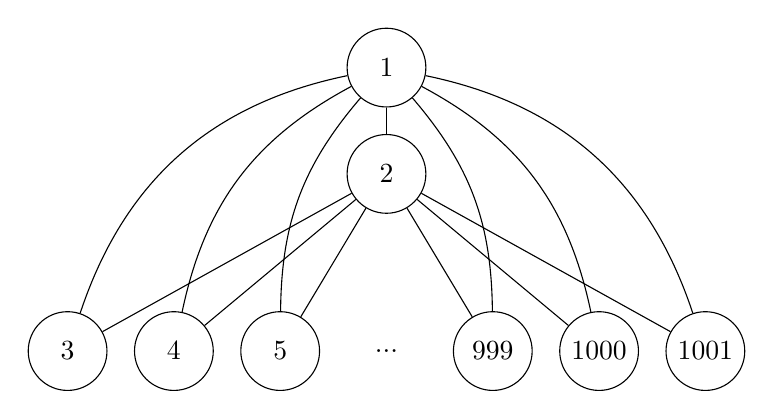
\begin{tikzpicture}[>=latex,scale=0.9]
            \begin{scope}[every node/.style={circle, draw = black,minimum size=10mm,inner sep=2pt}] 
                \node (1) at (0, 0) {1};
                \node (2) at (0, -1.5) {2};
                \node (3) at (-4.5, -4) {3};
                \node (4) at (-3, -4) {4};
                \node (5) at (-1.5, -4) {5};
                \node (7) at (1.5, -4) {999};
                \node (8) at (3, -4) {1000};
                \node (9) at (4.5, -4) {1001};
            \end{scope}
            \tikzset{e4c node/.style={circle,draw=none,minimum size=1.0cm,inner sep=0}}
            \node (6) at (0, -4) {...};
    
            \draw (1)--(2);
            \draw (2)--(3);
            \draw (2)--(4);
            \draw (2)--(5);
            \draw (2)--(7);
            \draw (2)--(8);
            \draw (2)--(9);
    
            \path
                (3) edge[-, bend left = 30] (1)
                (4) edge[-, bend left = 25] (1)
                (5) edge[-, bend left = 20] (1)
                (7) edge[-, bend left = -20] (1)
                (8) edge[-, bend left = -25] (1)
                (9) edge[-, bend left = -30] (1);
        \end{tikzpicture}
        \end{center}
    \end{enumerate}

    % Patryk
    \sol Koszt wykonania algorytmu Dijkstry dla spójnego grafu $n$-wierzchołkowego o $m$ krawędziach wynosi
    \answerss{$O(m\log{n})$ w implementacji z kopcem zupełnym}{$O(n\log{n}+m)$ w implementacji z kopcem Fibonacciego}{$O(n^2)$ w implementacji z kolejką dwumianową}{TAK}{TAK}{NIE}

     Złożoność algorytmu Dijkstry to $O(m\cdot\texttt{DecreaseKey}+n\cdot\texttt{DeleteMin})$. W każdym kopcu operacja \texttt{DeleteMin} ma koszt $O(\log{n})$, podobnie jak \texttt{DecreaseKey}, które jedynie w przypadku kopca Fibonacciego amortyzuje się do czasu stałego.

    \begin{enumerate}[\bf A.]
        \item Czas będzie $O(m\log{n}+n\log{n})$, ale ponieważ graf jest spójny, to ma co najmniej $\Omega(n)$ krawędzi, więc drugi składnik sumy nic nie wnosi do złożoności i odpowiedzią jest \texttt{TAK}.

        \item Wstawiając powyższe złożoności kopca Fibonacciego do wzoru otrzymamy dokładnie taką złożoność, odpowiedź to \texttt{TAK}.

        \item Złożoność jest taka sama jak w \textbf{A.} ($O(m \log n)$), a $m$ może być rzędu $n^2$, więc odpowiedź to \texttt{NIE}.
    \end{enumerate}

    % Jasiek
    \sol Wysokość drzewa ukorzenionego mierzymy liczbą krawędzi na najdłuższej ścieżce z korzenia do wierzchołka w tym drzewie. Dany jest spójny $n$-wierzchołkowy graf dwuspójny wierzchołkowo (tzn. bez wierzchołków rozdzielających) o co najmniej 4 wierzchołkach. Prawdą jest, że
    \answerss{wysokość każdego drzewa przeszukiwania wszerz w takim grafie jest mniejsza od $n / 2$}{wysokość każdego drzewa przeszukiwania w głąb w takim grafie jest większa od $n / 2$}{wysokość każdego drzewa przeszukiwania w głąb w takim grafie wynosi co najmniej $3$}{NIE}{NIE}{NIE}
    
    Kontrprzykładem w \textbf{A.} może być cykl 4-wierzchołkowy. W takim cyklu głębokość drzewa BFS jest równa $2 = \frac{n}{2}$ (niezależnie od wierzchołka startowego).
    
    Kontrprzykład do \textbf{B.} oraz \textbf{C.} narysowany jest poniżej (wierzchołek o numerze 1 jest korzeniem w drzewie, a DFS wchodzi najpierw do wierzchołka numer 2):
    \begin{center}
        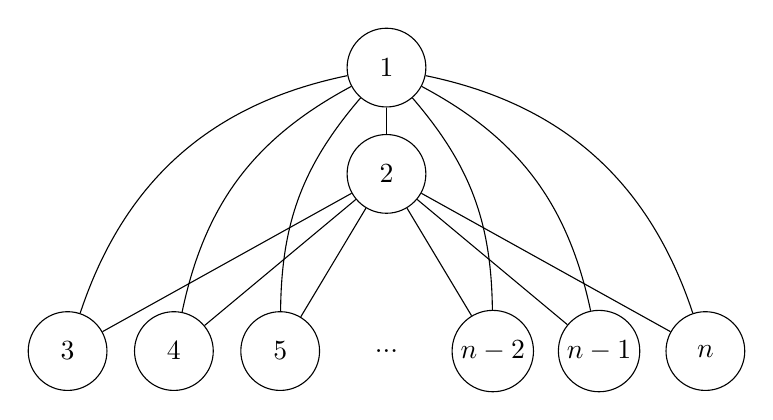
\begin{tikzpicture}[>=latex,scale=0.9]
            \begin{scope}[every node/.style={circle, draw = black,minimum size=10mm,inner sep=2pt}] 
                \node (1) at (0, 0) {1};
                \node (2) at (0, -1.5) {2};
                \node (3) at (-4.5, -4) {3};
                \node (4) at (-3, -4) {4};
                \node (5) at (-1.5, -4) {5};
                \node (7) at (1.5, -4) {$n - 2$};
                \node (8) at (3, -4) {$n - 1$};
                \node (9) at (4.5, -4) {$n$};
            \end{scope}
            \tikzset{e4c node/.style={circle,draw=none,minimum size=1.0cm,inner sep=0}}
            \node (6) at (0, -4) {...};
    
            \draw (1)--(2);
            \draw (2)--(3);
            \draw (2)--(4);
            \draw (2)--(5);
            \draw (2)--(7);
            \draw (2)--(8);
            \draw (2)--(9);
    
            \path
                (3) edge[-, bend left = 30] (1)
                (4) edge[-, bend left = 25] (1)
                (5) edge[-, bend left = 20] (1)
                (7) edge[-, bend left = -20] (1)
                (8) edge[-, bend left = -25] (1)
                (9) edge[-, bend left = -30] (1);
        \end{tikzpicture}
    \end{center}

    % Julia
    \sol Wysokość drzewa BST zawierającego 100 wierzchołków
    \answerss{wynosi co najmniej 49}{wynosi co najmniej 7}{wynosi co najwyżej 99}{NIE}{NIE}{TAK}

    Drzewo BST o największej wysokości to prosta z naniesionymi kolejnymi wierzchołkami, zatem wysokość takiego drzewa jest równa liczbie wierzchołków pomniejszonej o jeden (w naszym przypadku $99$).
    
    Drzewo BST z najmniejszą liczbą wierzchołków, to drzewo, w którym wierzchołki na każdym poziomie (oprócz ostatniego) mają po dwóch synów. Zatem wysokość takiego drzewa będzie wynosiła $\lfloor \log_2(n) \rfloor$, gdzie $n$ to liczba wierzchołków (w naszym przypadku $6$).

    % Julia
    \sol O drzewach AVL prawdą jest, że
    \answerss{największe drzewo AVL o wysokości 5 ma 64 wierzchołki}{najmniejsze drzewo AVL o wysokości 5 ma 20 wierzchołków}{każde drzewo czerwono-czarne jest AVL drzewem}{NIE}{TAK}{NIE}

    \begin{enumerate}[\bf A.]
        \item Największe drzewo AVL to po prostu największe drzewo BST, czyli drzewo posiadające dwóch synów na każdym poziomie. Zatem największe drzewo AVL o wysokości $h$ będzie posiadać $2^{h+1} - 1$ wierzchołków (czyli w naszym przypadku 63).

        \item Rozwiązanie tego podpunktu dość łatwo narysować na kartce, dokładając kolejno potrzebne wierzchołki. Można też skorzystać ze wzoru $M(h) = 1 + M(h-1) + M(h-2)$, gdzie $M(h)$ to minimalna liczba wierzchołków w drzewie AVL o wysokości $h$.

        \item Nie, ponieważ drzewo czerwono-czarne nie musi być zbalansowane, tak jak drzewo AVL.
    \end{enumerate}

    % Patryk
    \sol Do początkowo pustego drzewa BST wstawiamy kolejno elementy pewnej permutacji liczb $1,2,\ldots,16$. Liczba permutacji, dla których
    \answerss{dostaniemy drzewo o wysokości (czyli maksymalnej liczbie krawędzi na ścieżce od korzenia do liścia) równej 15, wynosi co najwyżej $2^{16}$}{dostaniemy drzewo o wysokości równej 3, wynosi co najmniej $2^{15}$}{w lewym poddrzewie korzenia będzie tylko węzeł z kluczem 1, wynosi co najmniej jeden miliard}{TAK}{NIE}{TAK}

    \begin{enumerate}[\bf A.]
        \item Żeby zbudować drzewo o takiej (maksymalnej) wysokości, w permutacji muszą występować kolejno największa lub najmniejsza aktualnie możliwa liczba, np. $16,1,2,3,15,4,14,13,12,5,6,11,...$. Na każdym kroku mamy wybór pomiędzy dwoma liczbami, więc takich permutacji będzie $2^{15} \leq 2^{16}$.

        \item Drzewo o wysokości 3 może mieć maksymalnie 15 elementów, więc jest 0 takich permutacji.

        \item Aby w lewym poddrzewie była tylko jedynka, pierwszym elementem permutacji musi być ,,2'', reszta może być losowo. Zatem takich permutacji jest $15!$. Wiemy że $7! > 1000 = 10^3$ oraz $15\cdot 14\cdot 13\cdot 12\cdot 11\cdot 10\cdot > 10^6$ więc $15! > 10^9$.
    \end{enumerate}

    % Grześ
    \sol W zbiorze AVL-drzew o 10 węzłach
    \answerss{istnieje drzewo o wysokości (czyli największej liczbie krawędzi od korzenia do liścia) równej 4}{każde drzewo ma wysokość co najmniej 3}{maksymalna różnica liczb węzłów poddrzew korzenia wynosi 5}{NIE}{TAK}{TAK}

    \begin{enumerate}[\bf A.]
        \item Minimalna liczba wierzchołków w AVL drzewie o wysokości 4 wynosi 12, więc mając 10 wierzchołków możemy uzyskać co najwyżej wysokość 3.

        \item Pełne drzewo binarne o wysokości 2 ma 7 wierzchołków, więc mając ich 10 możemy zbudować drzewo co najmniej o wysokości równej 3.

        \item Maksymalną różnicę dostaniemy, jeśli jednym poddrzewem korzenia będzie wierzchołek mający jednego syna, który jest liściem, a drugie poddrzewo korzenia będzie pełnym drzewem binarnym o wysokości równej 2. Wtedy lewe poddrzewo ma 2 wierzchołki, a prawe -- 7.
    \end{enumerate}

    \sol Niech $\Sigma = \{a, b\} $ będzie dwuznakowym alfabetem, a $s$ i $t$ słowami nad $\Sigma$ o długościach odpowiednio $m$ i $n$, gdzie $0 < m \leq n$. W algorytmie KMP wyszukiwania wzorca $s$ w tekście $t$
    \answerss
    {wszystkie wystąpienia słowa $s$ w słowie $t$ zostaną znalezione w czasie $O(n)$}
    {preprocessing zajmuje czas $\Omega (n)$}
    {każdy symbol ze słowa $t$ jest porównywany z co najwyżej jednym symbolem ze słowa $s$}
    {TAK}{TAK}{NIE}
    \textbf{A.} Algorytm KMP działa w czasie $O(n)$.

    \textbf{B.} Trzeba policzyć tablicę prefikso-sufiksów, co zajmuje czas liniowy.

    \textbf{C.} Nie musi tak być, np. mając $s=abab$ i $t=ababab$, prefikso-sufiks słowa $s$ wynosi 2, więc po każdym wystąpieniu wzorca w tekście cofniemy się o 2, więc niektóre symbole z $t$ porównamy dwa razy.

% COTO
    % Grześ
    \sol Dana jest funkcja
    \begin{cpp}
        int coto(int n) {
            if (n = 0)
                return 1;
            else if (n > 0)
                return coto(n - 1) + coto(-n);
            else
                return coto(n + 1) - 1;
        }
    \end{cpp}
    Przypisanie \cppinline{y = coto(x)} spowoduje, że będzie zachodzić zależność
    \answerss{$|y|\geq|x|$}{$y\leq1$}{jeśli $x=-2012$, to $y=-2011$}{NIE}{TAK}{TAK}
    
    Prześledźmy, co robi funkcja \cppinline{coto(x)}. Jeśli $x=0$, to \textbf{wyznacza} wartość 1. Jeśli $x<0$, to funkcja \textbf{oblicza} wartość $|x|\cdot(-1)+1=-|x|+1=x+1$. Jeśli $x>0$, to funkcja \textbf{przekazuje} wartość rekurencji $F_n=F_{n-1}-n+1$. Ostatecznie,
    $$
    \cppinline{coto(x)}=\begin{cases}
        1 & \text{gdy } x=0 \\
        \cppinline{coto(x-1)}-x+1 & \text{gdy } x>0 \\
        x+1 & \text{gdy } x<0
    \end{cases}=\begin{cases}
        \cppinline{coto(x-1)}-x+1 & \text{gdy } x>0 \\
        x+1 & \text{wpp.}
    \end{cases}
    $$

    \begin{enumerate}[\bf A.]
        \item Widzimy, że wstawiając za $x$ ujemną liczbę (np. $-5$) dostaniemy w wyniku liczbę większą o 1 (np. $-4$), czyli w module będzie to liczba mniejsza o 1, a więc fałsz.

        \item Dla liczb niedodatnich widać od razu. Dla liczb dodatnich można by policzyć tą rekurencję, ale można też rozpisać kilka pierwszych wyrazów ciągu: $(1,0,-2,-5,-9,\ldots)$. Już dla $x>2$ dostajemy liczby ujemne, a dla $x=0$ i $x=1$ coś nie większego od 1, czyli odpowiedź to \texttt{TAK}

        \item Widać od razu -- dla liczby ujemnej dostajemy liczbę większą o 1.
    \end{enumerate}

    PS. \textit{Istnieje w języku polskim niezbyt szczęśliwe tłumaczenie słowa ,,return'', jako ,,zwracać''. Jest to niezbyt zręczna kalka językowa bez specjalnego uzasadnienia. Zamiast mówić ,,funkcja zwraca wartość'' proponuję ,,funkcja \{wyznacza, oblicza, przekazuje\} wartość''.} Autor rozwiązania trzymał się konwencji poznanej na Wstępie do Programowania Imperatywnego autorstwa docenta Piotra Chrząstowskiego-Wachtla i zachęca, aby Czytelnik również się do niej stosował.
\end{solutions}
